% Chapter 4

\chapter{SYSTEM DESIGN} % All Chapter headings in ALL CAPS

\section{SYSTEM DATA STRUCTURES}

The system makes use of certain data structures for efficient performance and understandable abstraction. The email texts are periodically stored, processed and transformed in this architecture, as follows.
\subsection{TEXT ARRAY} 
The Spam and Ham email bodies are loaded into vectors of data type char, namely ‘$txt-array$’, which is used for initialising the input. These $txt-arrays$ are sent as input into the preprocessing software.

\subsection{MODIFIED TEXT ARRAY}
The content of this array is the result of modification of $txt-array$. The content of each $txt-array$ is converted to lowercase letters while also removing the punctuation marks. This new text, is loaded into the $modified-text-array$.

\subsection{TERM BY DOCUMENT MATRIX}
All $modified-text-arrays$ are passed through a tfidf vectorizer and the resultant vectors are stored in the form of a matrix in a Term By Document Matrix. The Matrix contains vectorized form of the text which shall be used for further processing, as processing numbers are easier than text.
          
\subsection{TRIPLET MATRIX <U,S,V>}
This composition is generated  by passing the Term by Document Matrix through a Single-Value-Decomposition factoring method. This generates three matrices, namely, U, S and V matrices, with matrix S being a diagonal matrix. These constructs are used for creating the feature set.

\subsection{REDUCE TERM BY DOCUMENT MATRIX}
Latent Semantic Feature Space is a method which is slightly different from the Latent Semantic Analysis, where each document is multiplied with the transpose of the ‘U’ matrix (rather than multiplying ‘S‘ also as done in LSA) to generate the Feature Set. Since, the size of the matrix U is very large, corresponding feature reduction is ensued. Top ‘k’ features are selected in the diagonal matrix, S, since it corresponds to both the term and documents of the Data Space. The corresponding rows in the U matrix, to these top k highest elements from the S matrix are used. This new matrix form the reduced term by document matrix and is used for generating the feature set.

\subsection{FEATURE SET}
Each document is done transformed with the TF*IDF vectorizer and is multiplied with transpose of reduced term by  document matrix. The resultant vectors are stored in a data construct called the feature set, which shall be used for training and testing the Neural Network.

\subsection{TRAINING AND TESTING SET}
The Feature is split in a 90-10 fashion for training and testing the neural network. The split is done in by randomly choosing 10\% of the data set (Ling-Spam Corpus provides the data set in a 10 part fashion which is pre-randomised).
        

\section{MODULE DESIGN}

\subsection{TF*ID VECTORIZER TOOL}
Using NLTK utilities, this tool is initialised to pre-process the natural language text, by removing stop words, tokenizing, stemming and vectorizing the text, in the same order as mentioned. It converts the tokens into vectors using TF*IDF algorithm.

\subsubsection{TEXT STEMMER}


For stemming, a Snowball stemmer is made use of. The initialization algorithm for this module is show below.

\begin{figure}[h]
\centering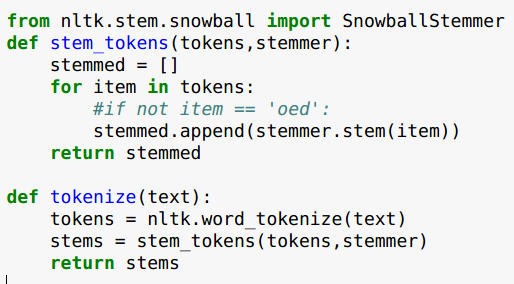
\includegraphics[width=0.8\linewidth]{vec.png}
\caption{Vectorizer}
\end{figure}

\subsubsection{TOKENIZER}


The tokenizer function is used to tokenize the text and to call the stemmer function. The pseudocode for the same is shown below.


\subsection{SINGLE VALUE DECOMPOSITION}
In linear algebra, the singular value decomposition (SVD) is a factorization of a real or complex matrix. It is the generalization of the eigendecomposition of a positive semidefinite normal matrix (for example, a symmetric matrix with positive eigenvalues) to any matrix via an extension of polar decomposition. This algorithm is used to reduce the dimensionality of the Term by document matrix.

$<U,S,V>=np.linalg.svd(D, full_matrices=0, compute_uv=1)$  

\subsection{TERM BY DOCUMENT MATRIX}
The resultant of the Single value decomposition poses to be a very large matrix which is tough to process later on. As explained before the U matrix is reduced by finding the K largest values in S matrix. The algorithm for the same is given below.

\begin{figure}[h]
\centering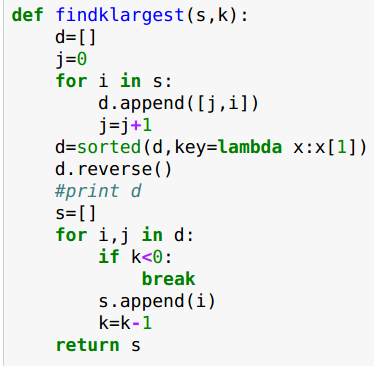
\includegraphics[width=0.6\linewidth]{findk.png}
\caption{Find K largest Rows}
\end{figure}

\subsection{CREATE DATASET}
Once the feature space is defined each document is processed using the feature space matrix (U’) to create the data set for testing and training the neural network. The algorithm for the same is given below.

\begin{algorithm}
\caption\textbf{{Creating Data Set}}
\begin{algorithmic}[1]
\Procedure{}
\State $s=u^T*tfidf.transform(s)$
\State \textbf{return} $s$
\EndProcedure
\end{algorithmic}
\end{algorithm}

\subsection{NEURAL NETWORK}
A simple feed forward neural network is used to classify the documents as spam and ham. The algorithm is designed by having two layers before the output layer, with the activation functions being “tanh” and “softmax” respectively. The optimizer function for the same is Stochastic Gradient Descent. 
The number of nodes in each layer is defined by the formula (Nprev-Nnext)/2.  

\section{CLASS DIAGRAM}

The class diagram of the spam classification system is shown in the figure. This diagram depicts the functions of various modules in the system clearly. It also shows the interaction between the modules of the system thereby providing a clear idea for implementation.

\begin{figure}[h]
\centering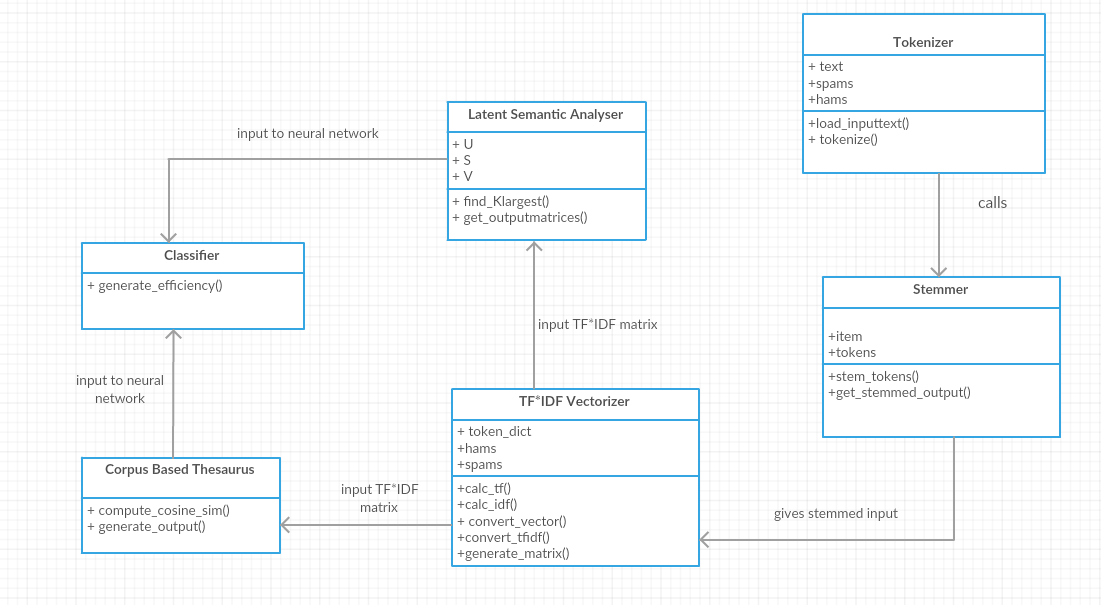
\includegraphics[width=1.0\linewidth]{class.png}
\caption{Class Diagram}
\end{figure}

\section{COMPLEXITY ANALYSIS}
\subsection{TIME COMPLEXITY}
The Time complexity of each module is shown in the table 4.1.

\begin{table}[]
\centering
\caption{Time Complexity}
\label{my-label}
\begin{tabular}{|l|l|l|}
\hline
\textit{\textbf{Sno}} & \textbf{Module}                       & \textbf{Complexity}    \\ \hline
1                     & TF*IDF Vectorizer                     & O(n\textasciicircum 2) \\ \hline
2                     & Single Value Decomposition            & O(n\textasciicircum 3) \\ \hline
3                     & Reduction of Term by Document Matrix  & O(n\textasciicircum 2) \\ \hline
4                     & Creating the Data Set                 & O(n)                   \\ \hline
5                     & Neural Network - Training and Testing & O(n\textasciicircum 3) \\ \hline
\end{tabular}
\end{table}
%\begin{figure}[h]
%\centering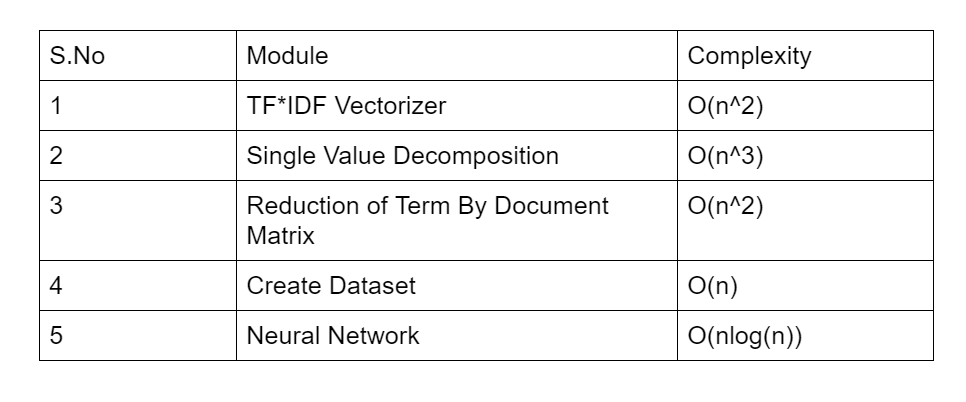
\includegraphics[width=1.0\linewidth]{complex.PNG}
%\caption{Time Complexity}
%\end{figure}

\subsection{COMPLEXITY OF THE PROJECT}
$1)$ The complexity of the system lies in dealing with words that are not present in the training set.


$2)$ The term by document matrix is computed for each word in the dataset.


$3)$ Words or sentences that are trained as spams but appear in ham emails reduce the overall efficiency of the system.


$4)$ In Corpus based Thesaurus,instead of checking co-occurence between just 2 words,we could determine a feature corresponding to relationship between n words.	